\section{Justificación e Importancia}

\subsection{Complejidad del Problema}

\cite{lenzerini:dataintegration}

\subsection{Ejemplo Motivante}

% flights
\newcommand{\flight}{\text{\it flight}}
\newcommand{\UScity}{\text{\it uscity}}
\newcommand{\national}{\text{\it national}}
\newcommand{\oneway}{\text{\it one-way}}
\newcommand{\onestop}{\text{\it one-stop}}
\newcommand{\flightPA}{\text{\it flight-to-pa}}
\newcommand{\onestopPA}{\text{\it onestop-to-pa}}
\newcommand{\fromNY}{\text{\it from-ny}}
\newcommand{\PA}{\text{PA}}
\newcommand{\NY}{\text{NY}}
\newcommand{\AL}{\text{AL}}
% end flights

Considere un sistema simple de información de vuelos que contiene información
sobre vuelos entre ciudades e información sobre qué ciudades están en los
Estados Unidos. Un sistema así puede ser descrito usando LAV con los dos servicios
abstractos $\flight(x,y)$ y $\UScity(x)$. El primero relaciona dos ciudades $x$ e $y$ si
hay un vuelo directo entre ellas, y el segundo dice si $x$ es una ciudad de
E.E.U.U.  o no. Para los servicios concretos, supongamos que las fuentes de
datos disponibles en Internet contienen la siguiente información:

\begin{enumerate}[--]
\item $\national(x,y)$ relaciona dos ciudades de E.E.U.U. conectadas por un vuelo directo,
\item $\oneway(x,y)$ relaciona dos ciudades conectadas por un vuelo de ida,
\item $\onestop(x,y)$ relaciona dos ciudades conectadas por un vuelo con una escala,
\item $\flightPA(x)$ dice si hay un vuelo directo desde $x$ a París,
\item $\onestopPA(x,y)$ relaciona $x$ y $y$ si hay un vuelo desde $x$ a París con una escala en $y$, y
\item $\fromNY(x)$ dice si hay un vuelo de Nueva York a $x$.
\end{enumerate}

Adicionalmente, los servicios concretos se describen con los siguientes
servicios abstractos:

\begin{alignat*}{1}
\national(x,y)\   &\qrule\ \flight(x,y),\,\UScity(x),\,\UScity(y)\,. \\
\oneway(x,y)\     &\qrule\ \flight(x,y)\,. \\
\onestop(x,z)\    &\qrule\ \flight(x,y),\,\flight(y,z)\,. \\
\flightPA(x)\     &\qrule\ \flight(x,\PA)\,. \\
\onestopPA(x,y)\  &\qrule\ \flight(x,y),\,\flight(y,\PA)\,. \\
\fromNY(x)\       &\qrule\ \flight(\NY,x)\,.
\end{alignat*}

Ahora supongamos que un usuario está interesado en construir un flujo de trabajo
capaz de recuperar los vuelos ida y vuelta con una parada hacia cualquier ciudad
en el mundo, tales que los vuelos puedan detenerse en cualquier ciudad.

\[ W(x,w,y,z) \qrule \UScity(x),\,\flight(x,w),\,\flight(w,y),\,\flight(y,z),\,\flight(z,x)\,. \]

La siguiente consulta conjuntiva representa el flujo de trabajo que define esta
solicitud en términos de servicios abstractos. El flujo de trabajo es definido
de manera que todo lo relacionado sobre el ligamiento de parámetros de
entrada/salida es resuelto. Así, cualquier instanciación de los servicios
abstractos en términos de los servicios concretos es una implementación válida
del flujo de trabajo. Las implementaciones corresponden a composiciones de
servicios concretos en las cuales un servicio concreto puede implementar uno o
más servicios abstractos del flujo, pero cada servicio abstracto puede ser
implementado por exactamente un servicio concreto. Por ejemplo, la siguiente
composición corresponde a una de estas implementaciones.

\[ I(x,w,y,z)\ \qrule\ \national(x,w),\,\flightPA(w),\,\oneway(\PA,z),\,\national(z,x)\,. \]

Sin embargo, las siguientes dos composiciones no son válidas.

\begin{alignat*}{1}
I'(x,w,y,z)\  \qrule\ &\national(x,y),\,\flightPA(y),\,\fromNY(z),\,\national(z,x)\,. \\
I''(x,w,y,z)\ \qrule\ &\onestop(x,y),\,\oneway(y,z),\,\national(z,x)\,.
\end{alignat*}

La primera composición no es válida porque asocia la variable del flujo $y$ a
las constantes \PA\ y \NY\ que denotan ciudades diferentes. En la otra mano, $I''$
no lo implementa porque el servicio concreto $\onestop(x,y)$ no recibe como entrada
o produce como salida la ciudad intermedia donde el vuelo se detiene y entonces
no es posible asegurarse de que esa ciudad esté asociada a la ciudad $w$ que es
retornada por el flujo de trabajo.

Estos ejemplos muestran que las instanciaciones correctas de un flujo deben
manejar constantes de manera que dos constantes distintas no sean asociadas
entre sí de manera directa o indirectamente vía transitividad, y que todos los
atributos que aparezcan en un \emph{join} o en la salida sean producidos por los
servicios concretos seleccionados.

Los parámetros QoS son modelados anotando los servicios concretos con utilidades
que caracterizan su comportamiento y que luego son agregados durante la
instanciación. Así, como se mencionó previamente, la mejor instanciación es la
que minimiza (o maximiza) la agregación de utilidades.

\subsection{Resultados Experimentales}

Se realizó un análisis empírico sobre tres experimentos. Todos los experimentos
fueron realizados en una máquina de escritorio con un CPU Intel Core 2 Duo de
2GHz y 4GB de memoria, y el tiempo fue medido con el comando de Unix
\emph{time}.

El objetivo de los experimentos es determinar el rendimiento de la propuesta con
condiciones variantes. El principal beneficio de la aproximación propuesta es
que se puede compilar la teoría lógica para una instancia del problema y luego
calcular todas las instanciaciones, o las mejores, cualquier número de veces. El
modelo de costos para conseguir mejores instanciaciones puede ser cambiado sin
necesidad de recompilar la teoría lógica. Por lo tanto, la complejidad en tiempo
de la aproximación es básicamente el tiempo para codificar el WIP como un
CNF más el tiempo para compilar el CNF en un d-DNNF y el tiempo para decodificar
los modelos. Los tiempos para codificar y decodificar son despreciables
comparados con el tiempo para compilar el CNF. Por esto, el enfoque es en el tiempo
necesario para compilar los problemas de los experimentos.

El primer experimento consiste de problemas para consultas para viajes aéreos.
Los servicios concretos son de la forma $V_i(x,y)\qrule\ \flight(x,y,\AL_i)$
donde $\AL_i$ es una
constante que denota el nombre de una aerolínea, y $\flight(x,y,\AL_i)$ relaciona las
ciudades $x$ e $y$ tales que hay un vuelo entre $x$ e $y$ servido por $\AL_i$.
Se supone que este servicio concreto retorna todos los vuelos entre dos ciudades
con una aerolínea específica. El flujo de trabajo tiene la forma

\[ W(x_1,\ldots,x_n)\ \qrule\ \flight(\PA,x_1,z),\,\flight(x_1,x_2,z),\,\ldots,\,\flight(x_n,\NY,z)\,. \]

\begin{figure}[t]
\centering
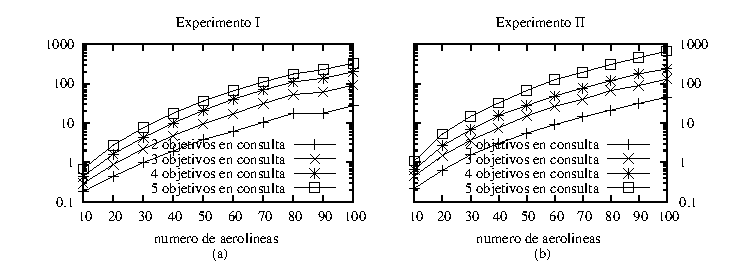
\includegraphics[width=1\textwidth]{graphics/plot1}
\caption{Tiempos de compilación para los experimentos I y II para diferentes
números de objetivos y de vistas. Los gráficos están en escala logarítmica, y el
tiempo es en segundos.}
\label{fig:plot1}
\end{figure}

El experimento incluye instancias para flujos de trabajo con 2 a 5 subobjetivos
y conjuntos de 10 a 100 servicios concretos. Los resultados para la compilación
son mostrados en el panel (a) de la figura ~\ref{fig:plot1}. Este es un gráfico en escala
logarítmica que sugiere comportamiento sub-exponencial. En cualquier caso, los
resultados muestran buen rendimiento dado que instancias realísticas del
problema (conjuntos de 100 aerolíneas con vuelos de cinco paradas) pueden ser
compiladas en 328 segundos. El tamaño en disco del d-DNNF para 100 aerolíneas y
vuelos con cinco paradas es 3,4MB. En este d-DNNF, el mejor modelo puede ser
computado en 0.29 segundos, y la enumeración de todos los modelos en 0.47
segundos.

En un intento de inducir crecimiento exponencial en el tamaño de compilación, en
el segundo experimento se agrega un segundo servicio concreto para cada
aerolínea. Esta modificación incrementa el número de instanciaciones válidas de
lineal a exponencial dado que cada tramo de un vuelo puede ser ahora instanciado
por dos servicios concretos y entonces un vuelo con $n$ tramos puede tener hasta
$2^n$ instanciaciones. Se corrió el compilador para instancias que comprendían
el mismo número de objetivos del flujo de trabajo y el número total de
servicios concretos. Los resultados graficados en escala logarítmica se muestran
en el panel (b) de la figura ~\ref{fig:plot1}.

Estas pruebas muestran buen rendimiento para este tipo de problemas, pero no
involucran servicios concretos con múltiples objetivos. Por lo tanto se
diseñó un tercer experimento que consiste de instancias no estructuradas y
generadas aleatoriamente. Cada instancia contiene tres variables por servicio
abstracto, diez variables distintas y diez constantes distintas, seis
objetivos en los flujos de trabajo, 2 a 5 objetivos en los servicios
concretos, y número de servicios variante. La probabilidad de que un argumento
de un servicio abstracto esté ligado a una constante es 50\%. Los resultados se
muestran en la figura ~\ref{fig:plot3}. El tiempo de compilación de estas instancias no
crece monótonamente dado que son generadas aleatoriamente. Lo mismo ocurre para
el tamaño de las teorías y los números de modelos. Por ejemplo, el d-DNNF para
un problema con 45 vistas cada una con 5 objetivos fue de tamaño 5,1Mb y tuvo
$1.26\times 10^8$ modelos. El tiempo para buscar el mejor modelo para este
d-DNNF es 0.46 segundos mientras que el tiempo para enumerar todos los modelos
es alredededor de 17 horas.

\begin{figure}[t]
\centering
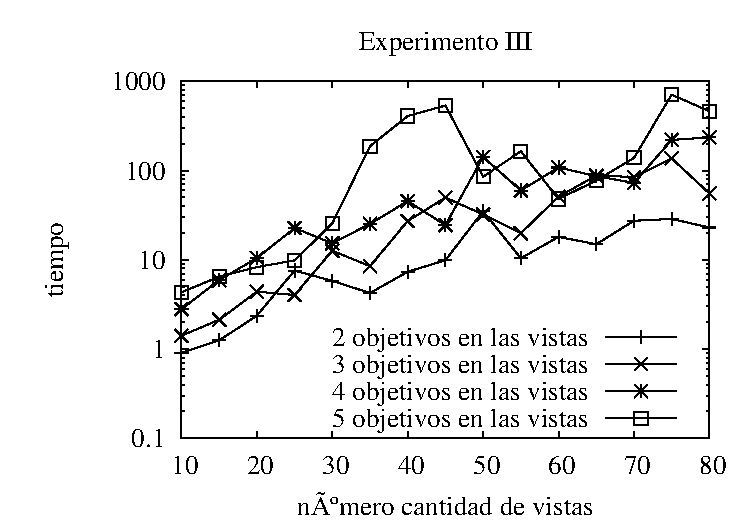
\includegraphics[width=.8\textwidth]{graphics/plot3}
\caption{Tiempos de compilación para el experimento III para diferentes números
de objetivos y de vistas. Los gráficos están en escala logarítmica, y el
tiempo es en segundos.}
\label{fig:plot3}
\end{figure}

Estos son experimentos preliminares, pero los resultados muestran que la
aproximación propuesta escala eficientemente para problemas con varios objetivos
y vistas. Se cree que estos resultados son alentadores y motivan a continuar
esta línea de investigación.
